\documentclass{beamer}
\usepackage{etex}
\usetheme{Antibes}
\usepackage{amssymb,amsmath,amsthm}
\usepackage{graphicx}
\usepackage{caption}
\usepackage{subfig}
\newcommand{\bn}{\begin{enumerate}[i)]}
\newcommand{\en}{\end{enumerate}}
\newcommand{\im}{\item}
\newcommand{\CPT}[1]{\large{\textbf{CHAPTER #1}}}
\newcommand{\ir}[1]{\textbf{Remark #1}}
\newcommand{\ith}[1]{\textbf{Theorem #1}}
\newcommand{\idf}[1]{\textbf{Definition #1}}
\newcommand{\iex}[1]{\textbf{Example #1}}

%\definecolor{cardinal}{rgb}{0.77, 0.12, 0.23}
%\usecolortheme[named=cardinal]{structure}
%\setbeamercolor{block title}{bg=cardinal,fg=black}
 \usepackage{tikz}
 \usetikzlibrary{patterns,snakes,plotmarks}
 \usepackage{multirow}
% \usetikzlibrary{shadows}
\usepackage{epstopdf}
\usepackage{nicefrac}
\usepackage{lmodern}
\usepackage{pgfplots}
\usepackage{qtree}
\newcommand*{\Scale}[2][4]{\scalebox{#1}{\ensuremath{#2}}}%
\DeclareCaptionLabelSeparator{horse}{:\,\,} % change according to your needs
\captionsetup{
  labelsep = horse,
  figureposition = bottom % used to get the correct vertical space between the figure and the caption
}
\setbeamertemplate{caption}[numbered]
\setbeamertemplate{items}[circle]
\setbeamertemplate{enumerate items}[square]
\theoremstyle{definition}
\newtheorem*{exs}{Examples}
\newtheorem{ex}{Example}
\newtheorem*{exc}{Exercise}
%\usepackage{booktabs}
\setlength{\parindent}{0pt}
%\setbeameroption{show notes}
 \setbeamerfont{note page}{size=\tiny}
%\setbeamertemplate{note page}[plain]
%\setbeameroption{show only notes}
\title{Math 629 - Survival Analysis \\ Chapter 1}
\author{Drew Lazar}
\institute{Ball State University}
\date{\today}

\begin{document}
\begin{frame}
    \titlepage
\end{frame}
\section{Chapter 1}
\begin{frame}\frametitle{Types of Censoring}
\bn
\item \textbf{Right Censoring:} An observation is \textbf{right censored} if the survival time is longer than its observed value. Some examples:
\bni
\item A five year study is conducted on how long it takes for machines to break down. A particular machine is observed from the start of the study but breaks down \textbf{after the study ends}.
\item Patients are followed for ten years after having a major heart attack. The response variable is time until death. A patient \textbf{withdraws} from the study after being followed for 2 years and moves to another country.
\item A study is done on smokers who have quit to see if they will resume smoking. Study participants are contacted by telephone. A participant changes his phone number, can not be reached and is \textbf{lost to follow-up}.
\en
\en
\end{frame}
\begin{frame} \frametitle{Types of Censoring cont'd}

\bn \setcounter{enumi}{2}
\item \textbf{Left Censoring:} An observation is \textbf{left censored} if the survival time is shorter than its observed value. For example, in following persons at risk until they become HIV positive.  For some patients we may not know the exact time becoming HIV, and therefore do not know exactly when the failure occurred.
\item \textbf{Interval Censoring:} An observation is \textbf{interval censored} if the event is known to occur in some interval. For example, a study is done to see the time until children can count to ten. The children are observed every 2 months. A child can count to ten at a follow-up time but couldn't count to ten at the previous visit.
\en
\end{frame}


\begin{frame}
\begin{columns}
    \begin{column}{0.48\textwidth}
        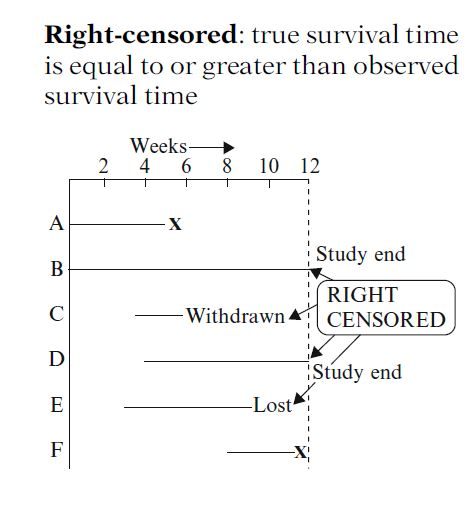
\includegraphics[width = \textwidth]{Ch1-RightCensor.JPG}
    \end{column}
    \hspace{-40pt}
    \begin{column}{0.48\textwidth}
         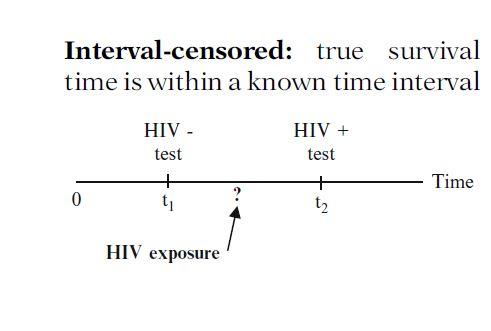
\includegraphics[width = \textwidth]{Ch1-IntervalCensor.JPG} \\
              \vspace{-20pt}
         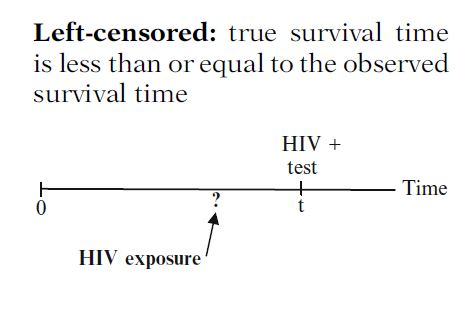
\includegraphics[width =\textwidth]{Ch1-LeftCensor.JPG}
    \end{column}
\end{columns}
\end{frame}
\begin{frame} \frametitle{Considerations about hazard rate}
\begin{block}{Hazard rate is dependent on time}
\begin{enumerate}
\item The hazard rate is dependent on the unit of measurement of time. For example, say $S$ is time measured in seconds and $T$ is time measure in minutes. Then
\begin{align*}
h(t) & = \lim_{\Delta t \to 0} \frac{P( t \leq T < t+ \Delta t|T \ge t)}{\Delta t} \\
 & = \lim_{\Delta s \to 0} \frac{P( s \leq S < s + \Delta s |S \ge s)}{\Delta (s/60)} \\
 &  = 60h(s)
\end{align*}
\end{enumerate}
\end{block}
\end{frame}

\begin{frame}\frametitle{Considerations about hazard rate (cont'd)}
\begin{block}{Other considerations about hazard rate}
\begin{enumerate}
  \setcounter{enumi}{1}
\item Relative rates of hazard are the same at any particular time.  For example, at any particular time (in seconds),~$s$, let $h(s,0)$ be the hazard for men (sex=0) and $h(s,1)$ be the hazard for women (sex=1). Then with $t$ the time in minutes,
    \[ \dfrac{h(t,0)}{h(t,1)} =  \dfrac{60 h(s,0)}{60 h(s,1)} = \dfrac{ h(s,0)}{ h(s,1)}
    \]
\item Can identify underlying distribution from hazard rate, for example, exponential has constant hazard, Weibull has proportional and monotonic hazard, lognormal has increasing than decreasing hazard, etc.
\item Can recover survival function from hazard rate.
\end{enumerate}
\end{block}
\end{frame}

\begin{frame}\frametitle{Hazard Functions of Different Distributions}
\begin{columns}
    \begin{column}{0.48\textwidth}
        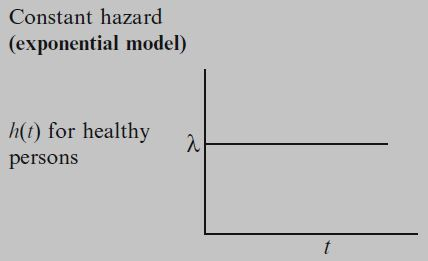
\includegraphics[width = \textwidth]{Hazards1.JPG} \\
           \includegraphics[width = \textwidth]{Hazards2.JPG}
    \end{column}
    \hspace{-10pt}
    \begin{column}{0.48\textwidth}
              \vspace{-20pt}
         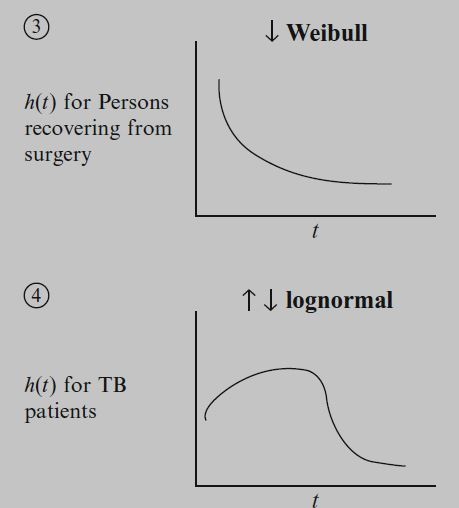
\includegraphics[width =\textwidth]{Hazards3.JPG}
    \end{column}
\end{columns}
\end{frame}



\begin{frame}
\frametitle{Ways to represent (right censored) survival data}
\begin{block}{First way to represent data }
\begin{columns}
    \begin{column}{0.48\textwidth}
        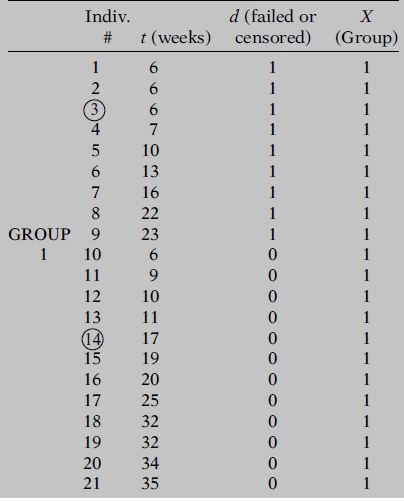
\includegraphics[width =\textwidth, height=6cm]{Ch1-leuk_dat_a.JPG}
    \end{column}
    \hspace{-10pt}
    \begin{column}{0.48\textwidth}
         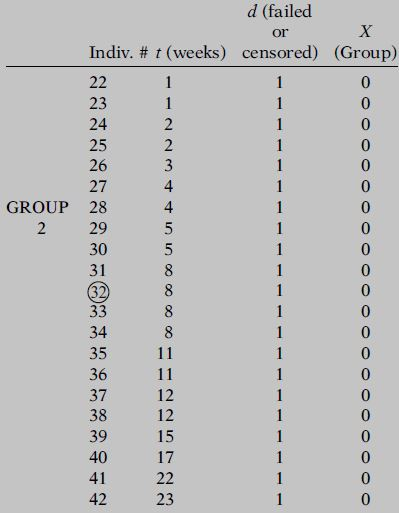
\includegraphics[width =\textwidth, height=6cm]{Ch1-leuk_dat_b.JPG}
    \end{column}
\end{columns}
\end{block}
\end{frame}

\begin{frame}
\frametitle{Ways to represent (right censored) survival data (cont'd)}
Consider the following data of times to remission of leukemia patients:
\begin{block}{Second way to represent data }
\begin{table}
\begin{center}
\begin{tabular}{l l}
Group 1 (n=21) treatment & Group 2 (n=21) placebo \\
 6, 6, 6, 7, 10, 13, 16, 22, 23, & 1, 1, 2, 2, 3, 4, 4, 5, 5,  \\
 6+, 9+, 10+, 11+, 17+, 19+, & 8, 8, 8, 8, 11, 11, 12, 12, \\
   20+, 25+, 32+, 32+, 34+, 35+ & 15, 17, 22, 23
\end{tabular}
\end{center}
\end{table}
Note: + denotes censored
\end{block}
\end{frame}

\begin{frame}
\frametitle{Ways to represent (right censored) survival data (cont'd)}
\begin{block}{Third way to represent data }
\begin{columns}
    \begin{column}{0.48\textwidth}
        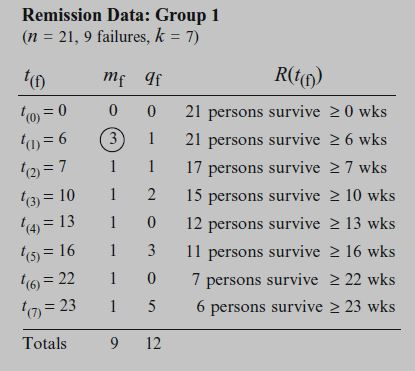
\includegraphics[width =\textwidth, height=6cm]{Ch1-leuk_data_a1.JPG}
    \end{column}
    \hspace{-10pt}
    \begin{column}{0.48\textwidth}
         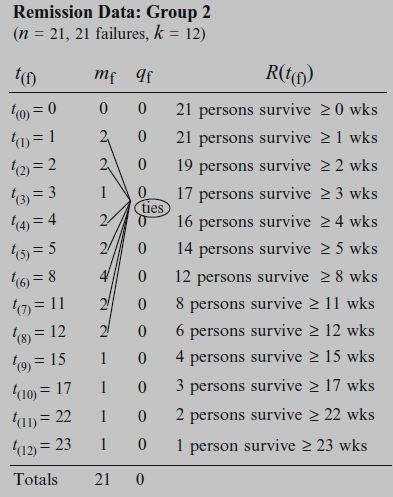
\includegraphics[width =\textwidth, height=6cm]{Ch1-leuk_data_b1.JPG}
    \end{column}
\end{columns}
\end{block}
\end{frame}

\begin{frame}
\frametitle{Ways to represent (right censored) survival data (cont'd)}
\begin{block}{Fourth way to represent data - Counting Process (CP) format}
\begin{columns}
    \begin{column}{0.48\textwidth}
        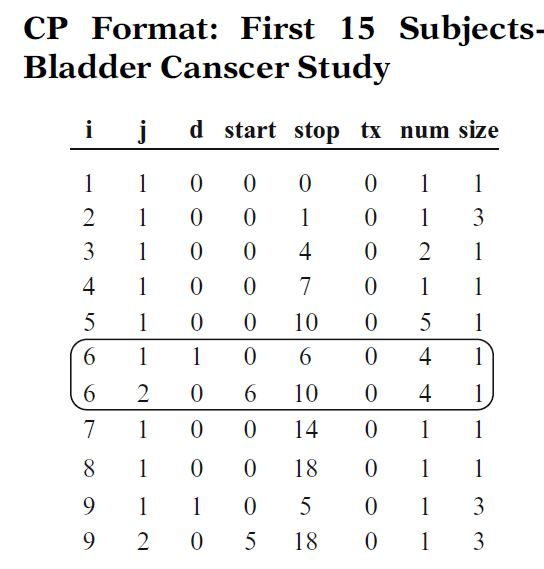
\includegraphics[width =\textwidth, height=5.5cm]{Ch1-CPFormat_1.JPG}
    \end{column}
    \hspace{-10pt}
    \begin{column}{0.48\textwidth}
         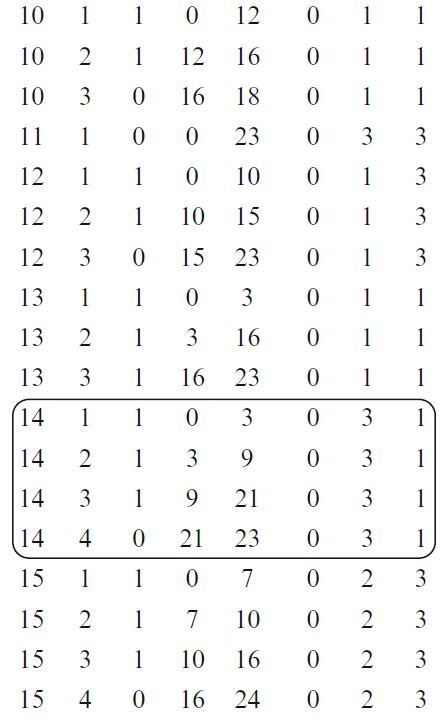
\includegraphics[width =\textwidth, height=5.5cm]{Ch1-CPFormat_2.JPG}
    \end{column}
\end{columns}
\end{block}
\end{frame}

\begin{frame}
\frametitle{Ways to represent (right censored) survival data (cont'd)}
\begin{block}{Fourth way to represent data }
\begin{itemize}
\item This data is the the recurrence of bladder cancer tumors after transurethral surgical excision.
\item Covariates are tx (0 or 1), num and size. Only tx=0 is included here.
\item $i$ is the subject, $j$ is the number of the event for the subject.
\item $d$ is censoring status, \textbf{start} is when event starts, \textbf{stop} is last time of observation of event.
\item For subject 6, two events are observed.
\begin{enumerate}[i.]
\item The first tumor starts at time 0 and stops (excised) at time 6.
\item The second tumor starts at time 6 and the observation is censored at time 10.
\end{enumerate}
\end{itemize}
\end{block}
\end{frame}

\begin{frame}
\frametitle{Kaplan Meier Estimates of Survival}
 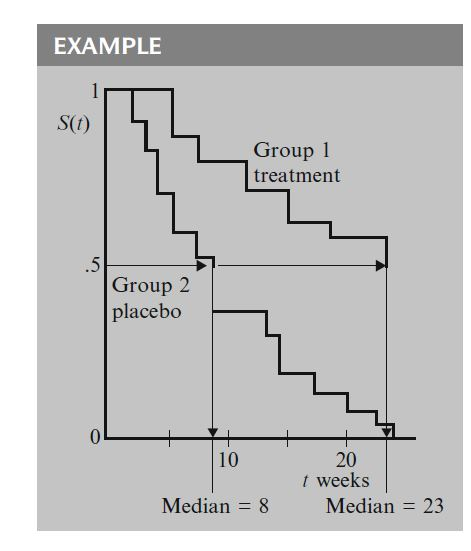
\includegraphics[width =\textwidth, height=5.5cm]{Ch1_estsurv.JPG}
 \end{frame}

\begin{frame}
\frametitle{Remission Data with LogWBC (Confounding Example)}
 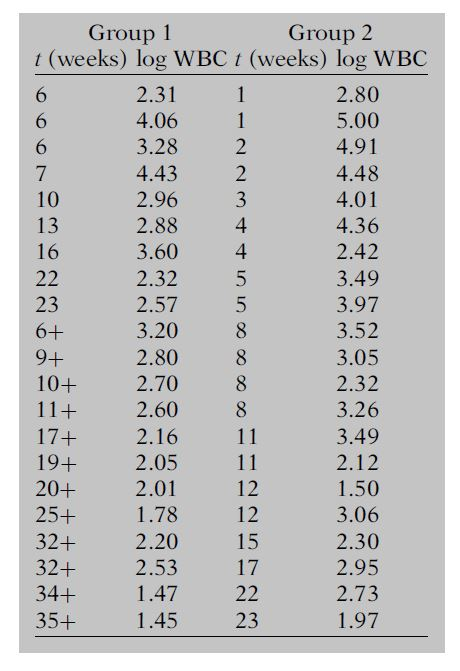
\includegraphics[width =\textwidth, height=6.5cm]{Ch1-RemissionwLogwbc.JPG}
 \end{frame}

\begin{frame}
\frametitle{Confounding Example}
 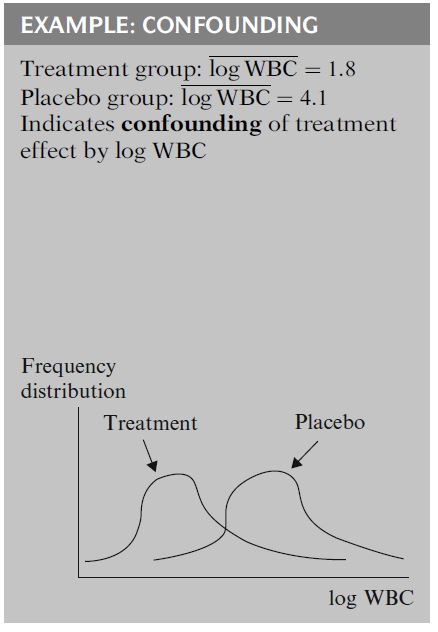
\includegraphics[width =\textwidth, height=6.5cm]{Ch1_Confound.JPG}
 \end{frame}

\begin{frame}
\begin{block}{Remark 1.4 - Confounding}
\begin{itemize}
\item We see the distribution of logWBC for the Treatment group and for the Placebo group.
\item The Placebo group tends to have higher logWBC with the mean logWBC for Treatment of 1.8 and the the mean logWBC for Placebo of 4.1.
\item Thus, if lower logWBC correlates with greater survival times, the effect of the treatment in creating greater survival times might be from this correlation rather than the effect of the treatment in itself.
\item In this case, the effect of treatment is \textbf{confounded} by the effect of treatment.
\item Confounding is dealt with by including secondary variables in semi-parametric models and parametric models.
\end{itemize}
\end{block}
\end{frame}


\begin{frame}
\frametitle{Interaction Example}
 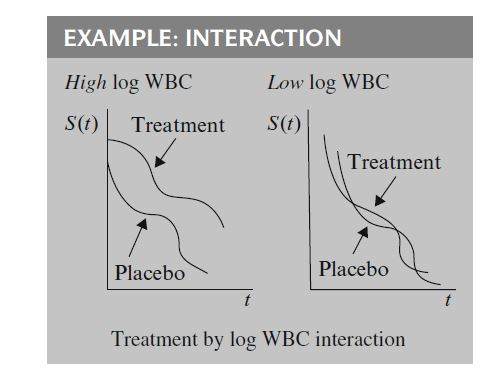
\includegraphics[width =\textwidth, height=6.5cm]{Ch1_Interact.JPG}
 \end{frame}


\begin{frame}
\begin{block}{Remark 1.4 - Interaction}
\begin{itemize}
\item We see the affect of Treatment depends on the level of logWBC.
\item For high logWBC Treatment has a positive effect on survival probabilities.
\item For low logWBC Treatment does not have a significant effect on survival probabilities.
\item Interaction is dealt with by 1) partitioning data on different levels of the secondary variable or 2) by including interaction terms in semi-parametric and parametric models.
\end{itemize}
\end{block}
\end{frame}


\begin{frame}
\frametitle{Assumptions about (right) censoring}
\begin{block}{Definition 1.9 - Random Censoring and Independent Censoring}
\begin{itemize}
\item \textbf{Random censoring} means that subjects who are censored at
time $t$ are representative of all the study subjects who remained at risk at time $t$ with respect to their survival experience. Thus, the failure rate for subjects who are
censored is assumed to be equal to the failure rate for subjects who remained in the risk set who are not censored.
\item \textbf{Independent censoring} means within any subgroup of interest, the subjects who are censored at time $t$ should be representative of all the subjects in that subgroup who remained at risk at time $t$ with respect to their survival experience. Thus, censoring is independent provided that it is random within any subgroup of interest.
\end{itemize}
\end{block}
\end{frame}



\begin{frame}
\frametitle{Assumptions about censoring}
\begin{block}{Example 1.1}
Consider a population with two groups - Group A and Group B.
\begin{center}
\textbf{Group A}
\begin{tabular}{ c c c c }
 Time & \# at risk & \# events & \# survived \\ \hline
 0-3 yrs & 100 & 20 & 80 \\
 3–5 yrs &  40 & 5 & 35
\end{tabular} \\
40 left study at the end of 3 years
\end{center}
\begin{center}
\textbf{Group B}
\begin{tabular}{ c c c c }
 Time & \# at risk & \# events & \# survived \\ \hline
 0-3 yrs & 100 & 40 & 60 \\
 3–5 yrs &  50 & 10 & 40
\end{tabular} \\
10 left study at the end of 3 years.
\end{center}
\end{block}
Assuming independent censoring summarize the 3 and 5 year survival experiences of both groups.
\end{frame}

\begin{frame}
\frametitle{Assumptions about censoring (cont'd)}
\begin{block}{Example 1.1}
Consider the entire population.
\begin{center}
\textbf{All}
\begin{tabular}{ c c c c }
 Time & \# at risk & \# events & \# survived \\ \hline
 0-3 yrs & 200 & 60 & 140 \\
 3–5 yrs &  90 & 15 & 75
\end{tabular} \\
50 left study at the end of 3 years.
\end{center}
\end{block}
If we assume independent censoring, do we have random censoring?
\end{frame}

\begin{frame}
\frametitle{Assumptions about censoring (cont'd)}
\begin{block}{Remark 1.4 - Random vs. Independent Censoring}
\begin{itemize}
\item Random censoring is a stronger condition than independent censoring.
\item Independent censoring only applies to groups of interest and random censoring applies to every subgroup including the entire data set.
\item Independent censoring is random censoring conditional on each level of covariates.
\item We only need and assume independent censoring for our covariates of interest.
\end{itemize}
\end{block}
\end{frame}


\begin{frame}
\frametitle{Assumptions about censoring (cont'd)}
\begin{block}{Remark 1.5 - Informative vs. NonInformative Censoring}
\begin{itemize}
\item \textbf{Non-informative censoring} occurs if the distribution of survival times ($T$) provides no
information about the distribution of censorship times ($C$), and vice versa. Otherwise, the
censoring is \textbf{informative}.
\item Independent censoring commonly fails when there is a drug side-effect that causes patients to drop out. In this case, those in the treatment group are not being censored at ``random'' and if we assume independent censoring then we are overestimating the survival experience of the treatment group. We assume independent censoring in this course.
\end{itemize}
\end{block}
\end{frame}

\end{document} 